\section{问题一模型建立与求解}

\subsection{问题一分析}

问题一给定单日负载、光伏预测及电价，并要求在零时一次性形成144个10分钟时段的购电计划，日末储电量恢复到日初水平。其关键是决定电量在同一时段内如何分配，以及通过电池向后续时段转移多少电量。低价购电未必立即用于负载，光伏富余也可补充储能；相反，高价时段是否放电取决于当时缺口、剩余电量及后续补能机会。

本文把附件1的已给曲线视为本问确定输入，先求解购电与储能的联合线性规划，为后续不确定条件下的采购提供共同物理基础。已有日前微网调度研究\cite{kong2016,silva2020}支持这一建模结构，本题只保留外网、光伏、负载和储能，不引入题目未给出的其他发电设备、售电收入或寿命折旧。确定性结果解释的是在给定输入下如何调度，不能作为未知实际负载时已经掌握完美信息的证明。

\subsection{问题一模型建立}

\subsubsection{决策变量与购电目标}

按统一物理索引$t=0,\ldots,143$，定义计划购电$g_t$、电池外侧充电$c_t$、电池外侧放电$d_t$和时段初储电量$e_t$，单位均为kWh。净负荷为$n_t=(L_t-R_t)\Delta t$，可以为负，负值表示光伏超过当期负载。购电按时段电价$p_t$收费，因此目标为
\begin{equation}
 \min_{g,c,d,e}\quad C_1=\sum_{t=0}^{143}p_tg_t.
 \label{eq:q1_objective}
\end{equation}
这里$g_t$已是10分钟电量，费用计算不再乘一次$\Delta t$。目标只含赛题要求支付的外购电费；免费弃余、已有电池和光伏均不额外产生本问未给定的收费项目。

\subsubsection{供需、储能与日末约束}

在任一时段，外网采购与电池放电至少补足净负荷及充电需求：
\begin{equation}
 g_t+d_t-c_t\ge n_t.
 \label{eq:balance}
\end{equation}
令$w_t=g_t+d_t-c_t-n_t\ge0$，即可改写为电量平衡等式。$w_t$表示未消纳的富余量，不能解释为向外网售电。

电池状态沿时间传递：
\begin{equation}
 e_{t+1}=e_t+\eta_cc_t-\frac{d_t}{\eta_d},
 \qquad \eta_c=\eta_d=0.9.
 \label{eq:soc}
\end{equation}
充电量$c_t$在电池外侧计量，只有$0.9c_t$进入电池；要对外输出$d_t$，内部需要消耗$d_t/0.9$。因此不能将充、放电项都乘0.9，也不能把完整往返效率误当为90\%。

容量和功率约束为
\begin{equation}
 E_{\min}\le e_{t+1}\le E_{\max},\qquad
 0\le c_t,d_t\le U,
 \quad E_{\min}=1200,\quad E_{\max}=10800,\quad U=5000/6.
 \label{eq:limits}
\end{equation}
储电量下限防止过度放电，上限防止过度充电；$U$由5000 kW乘$1/6$小时得到，分别限制一个时段可输入、输出的外侧电量。另有
\begin{equation}
 g_t\ge0,\qquad e_0=e_{144}=6000.
 \label{eq:terminal_q1}
\end{equation}
非负购电排除反向售电，首末相等排除通过额外消耗初始库存制造的单日账面节费。模型由线性目标、线性等式和不等式组成，可直接作为LP求解。

\subsubsection{免费弃余条件下的充放电互斥证明}

通常可用二进制变量禁止同时充放电，但本题免费弃余条件使其并非必要。若某可行解在时段$t$有$c_t,d_t>0$，取
\begin{equation}
 \varepsilon=\min\{c_t,d_t/(\eta_c\eta_d)\},\qquad
 c'_t=c_t-\varepsilon,\quad
 d'_t=d_t-\eta_c\eta_d\varepsilon.
 \label{eq:q1_remove_simultaneous}
\end{equation}
变换后至少有一种动作变为零，充放电量均不增大，因此不破坏功率上下界。同时
\[
 \eta_cc'_t-d'_t/\eta_d=\eta_cc_t-d_t/\eta_d,
\]
故全部储电轨迹与首末约束保持不变。供需约束左端增加$(1-\eta_c\eta_d)\varepsilon\ge0$，可将新增富余弃置，原购电量及费用无须增加。对所有同时充放电时段依次变换，得到满足互斥且费用不高于原解的方案。因此至少存在一组充放电互斥的最优解，无需为该条件额外引入整数变量。

程序在充放电总量上加入$10^{-7}$元/kWh的数值破同解项，以减少求解器返回无意义循环的可能；统计实际费用时剔除该项。以上证明依赖允许免费弃余，不能不加条件地推广到存在弃电罚金或必须消纳的其他问题。

\subsubsection{跨时段储能的经济条件}

若低价时段从外网购电并储存，要在高价时段对外输出1 kWh，低价段需购入$1/(\eta_c\eta_d)$ kWh。因此在忽略容量、功率及其他机会成本时，纯购电套利的必要盈利条件为
\begin{equation}
 p_h>\frac{p_\ell}{\eta_c\eta_d}=\frac{p_\ell}{0.81}.
 \label{eq:arbitrage}
\end{equation}
该式解释电池为何偏向低价补能、高价替代购电，但不足以单独确定完整计划。例如预期午间光伏可充满电池时，凌晨继续充电可能占用本可容纳免费光伏的容量；临近日末则还须为6000 kWh终值补能。完整LP同时处理这些跨时段竞争。

\subsection{问题一求解}

\subsubsection{求解步骤与结果核对}

首先按照统一时间映射读取附件1，将功率乘$\Delta t$得到净需求及单段充放电上限；然后以式\eqref{eq:soc}组装相邻状态的稀疏约束矩阵，加入购电、功率、容量和首末约束，由HiGHS求解。最后从未四舍五入的变量计算费用与汇总电量，核对144段供需平衡、储电递推、容量和功率界以及单段互斥。工作簿按原模板的源样本列序填写，论文指定时段则通过同一个物理索引取数。

计算得到全天计划购电量59482.6990 kWh、购电费35126.9486元。无储能基准逐时购买$[n_t]_+$，费用为48052.05元，因此采用储能节省12925.10元，节费率为26.90\%。电池外侧累计充电20740.67 kWh、放电16799.94 kWh，满足
\[
 \eta_c\sum_tc_t=\sum_td_t/\eta_d,
\]
与$e_0=e_{144}=6000$ kWh一致。充放电外侧累计量不相等，差额来自效率损耗，不是储能平衡错误。

\begin{table}[htbp]\centering\small\caption{问题1指定时段与全天购电结果（电量单位：kWh）}\label{tab:q1-purchase}\begin{tabularx}{\linewidth}{lRlRlR}
\toprule
时间段 & 购电量 & 时间段 & 购电量 & 时间段 & 购电量\\
\midrule
10:00--10:10 & 0.00 & 12:00--12:10 & 480.41 & 14:00--14:10 & 0.00\\
16:00--16:10 & 445.43 & 18:00--18:10 & 531.89 & 20:00--20:10 & 0.00\\
\midrule
全天购电量 & 59482.70 & \multicolumn{2}{c}{全天购电费（元）} & \multicolumn{2}{r}{35126.95}\\
\bottomrule
\end{tabularx}\end{table}
\begin{table}[htbp]\centering\small\caption{问题1储能充放电及首末电量（单位：kWh）}\label{tab:q1-battery}\begin{tabularx}{\linewidth}{lRRlRR}
\toprule
时间段 & 充电量 & 放电量 & 时间段 & 充电量 & 放电量\\
\midrule
00:00--04:00 & 4500.00 & 0.00 & 04:00--08:00 & 833.33 & 6365.84\\
08:00--12:00 & 4787.96 & 1703.00 & 12:00--16:00 & 5286.04 & 91.10\\
16:00--20:00 & 0.00 & 5780.13 & 20:00--24:00 & 5333.33 & 2859.87\\
\midrule
0:00储电量 & \multicolumn{2}{r}{6000.00} & 24:00储电量 & \multicolumn{2}{r}{6000.00}\\
\bottomrule
\end{tabularx}\end{table}

表\ref{tab:q1-purchase}中的全天购电量包含为负载和储能安排的所有外购电，表\ref{tab:q1-battery}则按六个物理四小时区间汇总充放电。某个四小时区间内两项均为正，表示其中不同10分钟时段分别充电或放电，不违反单时段互斥。

\subsubsection{调度结构与能量收支}

图\ref{fig:q1}将购电、充放电、SOC及电价对齐展示，用来判断电池如何在价格和净需求变化时转移电量。原始LP未包含爬坡、启停或平滑约束，因此保留其分段动作，不对最优结果额外平滑后再声称仍然最优。

\begin{figure}[htbp]\centering
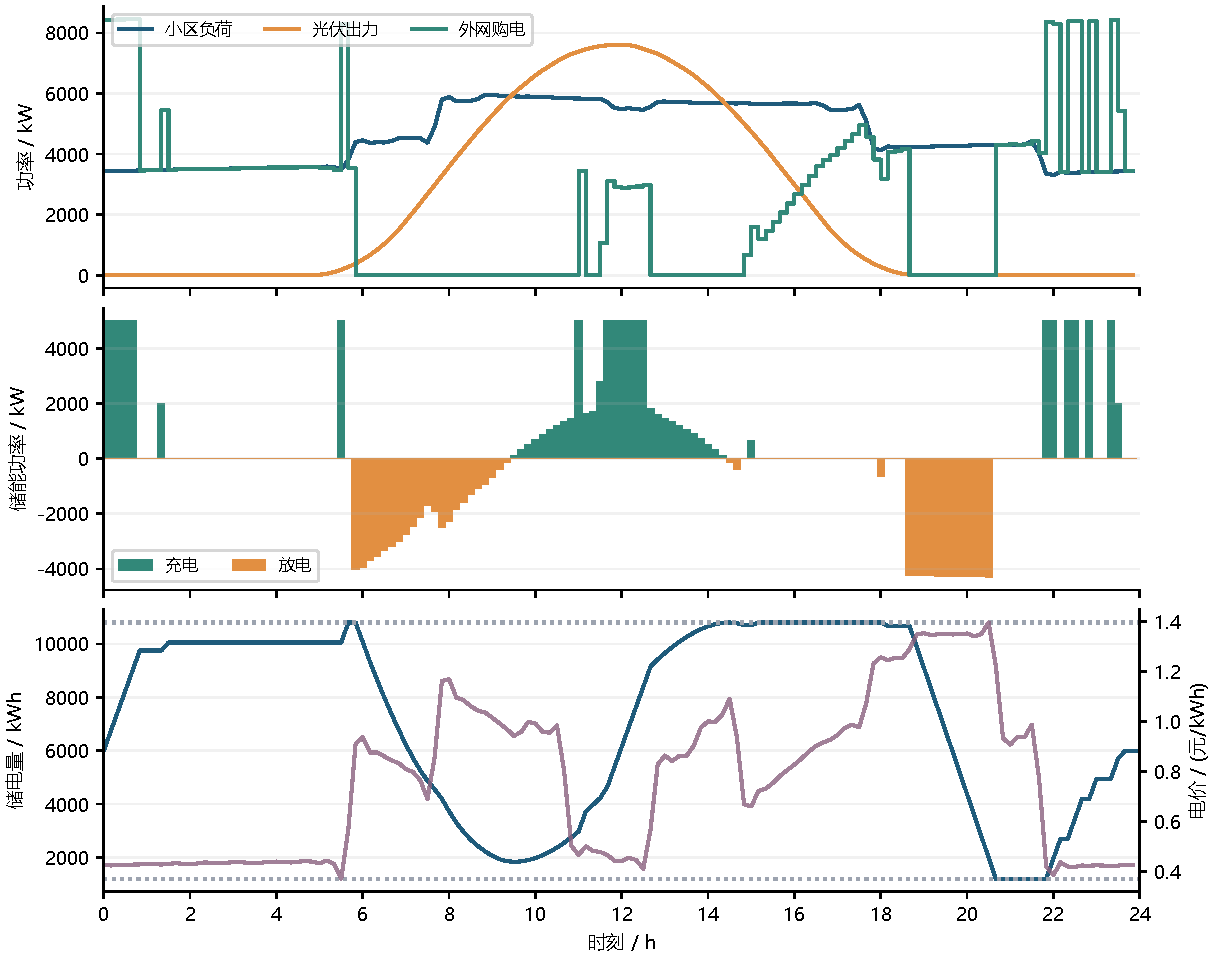
\includegraphics[
    width=0.90\linewidth,
    height=0.60\textheight,
    keepaspectratio
    ]{figures/results/q1_dispatch.pdf}
\caption{问题一购电、充放电、储电量及电价的日内对应关系}
\label{fig:q1}
\end{figure}

图\ref{fig:q1-energy-heatmap}把六个四小时区间的购电、光伏、负载、充电和放电量对齐展示，格内标注原始累计电量，便于与题目汇总表核对。下方平均库存另用独立色标，按区间内24段$(e_t+e_{t+1})/2$的平均计算，不与流量混作同一统计量。

\begin{figure}[htbp]\centering
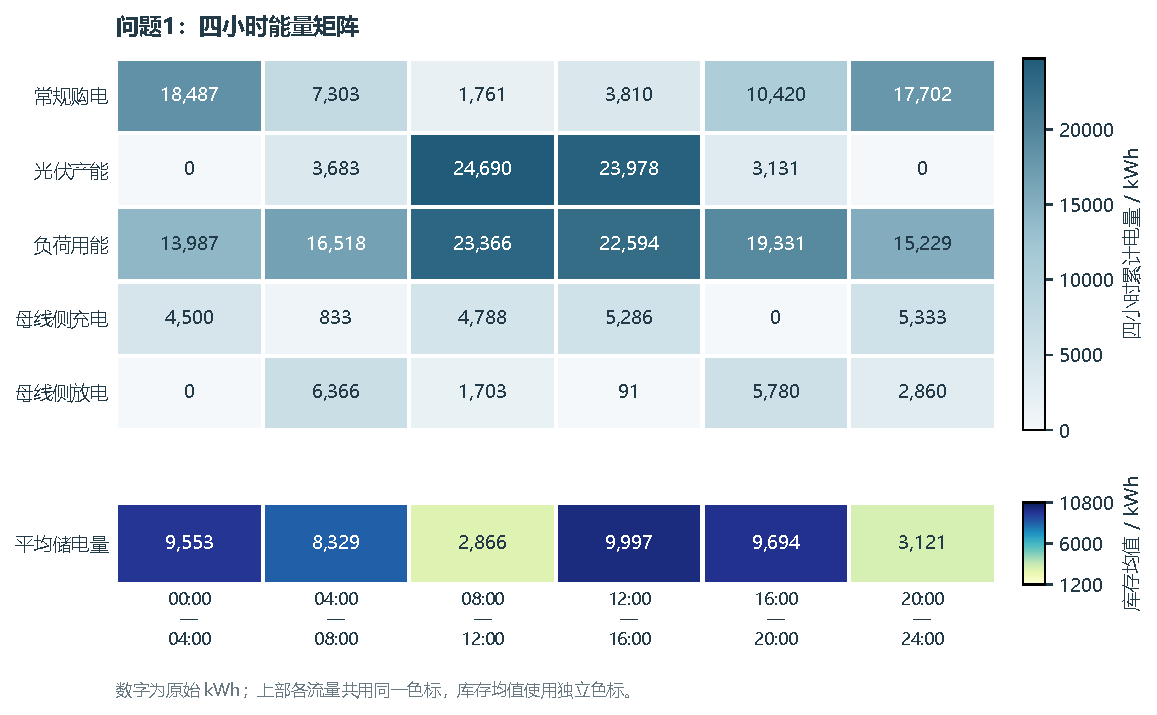
\includegraphics[width=0.94\linewidth]{figures/results/q1_energy_heatmap.pdf}
\caption{问题一六个物理四小时区间的累计电量与平均库存；流量共用色标，库存另设色标，标注单位均为kWh}
\label{fig:q1-energy-heatmap}
\end{figure}
\FloatBarrier
